
\hypertarget{secrets_after_installation}{}
\section{After installation}
\index{secrets!after installation}

At the top of the screen there is a Main menu (1) and two toolbars: the top toolbar is the \textit{main toolbar (2)}
and the bottom task bar is the \textit{\RR{} toolbar (3)}.

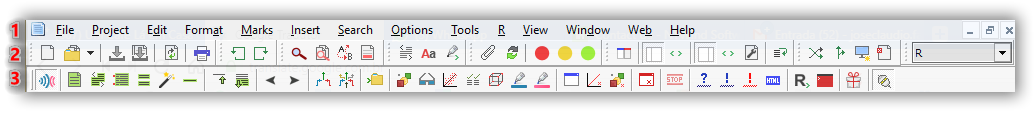
\includegraphics[scale=0.50]{./res/parts_02.png}

%Now, on the R main menu, click on the icon \textit{Configure/Permanent (Rprofile.site)}
%(\textit{\htmladdnormallink{see a very recurrent FAQ}{\#faq\_trpaths}}). You should have administrator rights to modify this file.
%If you do not have administrator rights, you should click on temporary,
%which will allow you to configure Tinn-R only for the current section.
%Bear in mind that if the packages \texttt{TinnR}, \texttt{svSocket} and \texttt{formatR} are not installed
%on your computer some of Tinn-R's advanced features will not work.
%
%\includegraphics[scale=0.50]{./res/secrets_configure.png}

%The \texttt{Rprofile.site} is a file which gives \RR{} (on startup) instructions on paths to find mirrors,
%packages to open and so forth. When clicking at that icon it saves on \texttt{Rprofile.site} instructions
%(a small but necessary script) to make the connection of Tinn-R with \RR{} more efficient.

If your version is the same or above 3.0.1.0, Tinn-R does not require any special configuration.
That is, the program is ready to be used. One important thing to be done before using it:
set a \RR{} mirror as close as possible to where you work. For that, first click on \texttt{CTRL + F8}.
This opens the \texttt{Tools} window, then click on \texttt{R/Mirrors}.
Select the \RR{} mirror and push the button that shows an hourglass in the taskbar.
The chosen repository will be the new default for all actions dependent repository
(install packages, upgrade packages, etc).

The second step is connecting Tinn-R with \RR{}. Look at the \textit{\RR{} toolbar}.
Almost at the right end you will see two icons together: one is the \RR{} symbol and the second is like a green television screen:

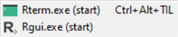
\includegraphics[scale=0.50]{./res/secrets_connecting.png}

The first connects Tinn-R to \texttt{\RR{} Console} (32 or 64 bit), also called \texttt{Rgui},
the second with \texttt{Rterm}. With Tinn-R the Rgui should be used only when you need heavy and intensive processing;
otherwise, you should always use Rterm, which is a lot more much friendly, having many editorial features of Tinn-R editor.
However it consumes more computer resources. Click on that little screen as soon as the connection with \RR{} is made.
That screen will become red and Rterm will appear on a window by itself. You can move that window across Tinn-R main
window and dock it either at the left, right or bottom side.

The best location will depend on the size of your computer screen. To do so, just put the mouse on the blue strip
at the top of Rterm window, click the left button of the mouse and move.
To dock it at either side just pull it closer and closer to the chosen side and then, bingo,
you will see how it becomes when docked. We like to use Tinn-R with two monitors:
the editor docked in one and the Rterm (or Rgui) interface in other.
It is a very comfortable and productive arrangement.
You should follow the same procedure to dock the \texttt{Tools} window.

Since \RR{} computer language is an interpreted one, each command given gets its answer right away,
therefore the most used command in Tinn-R is the \texttt{send line} which sends the command line to be interpreted by \RR{}.
You will see the answer to the command at Rterm or Rgui window.
This command appears at the bottom icon bar, the sixth box, the one with just one line.

\includegraphics[scale=0.50]{./res/secrets_sendline.png}

You just have to click there and the line is sent to \RR{}. Even though this is a nice way to do it,
there is a faster way to send a line to \RR{}. First, click on Options/Shortcuts/Keystrokes/Hotkeys (map) at the Main menu and then on
\htmladdnormallink{Hotkeys (operational system)}{\#working\_hotkeys}.
On the open window click on the line \texttt{send line} to select it.
Then go to the \texttt{Manager} button, click there and then press (for example, \texttt{Ctrl + \textbackslash{}}),
then click on the bottom bar the button \texttt{OK} and then set all to on.

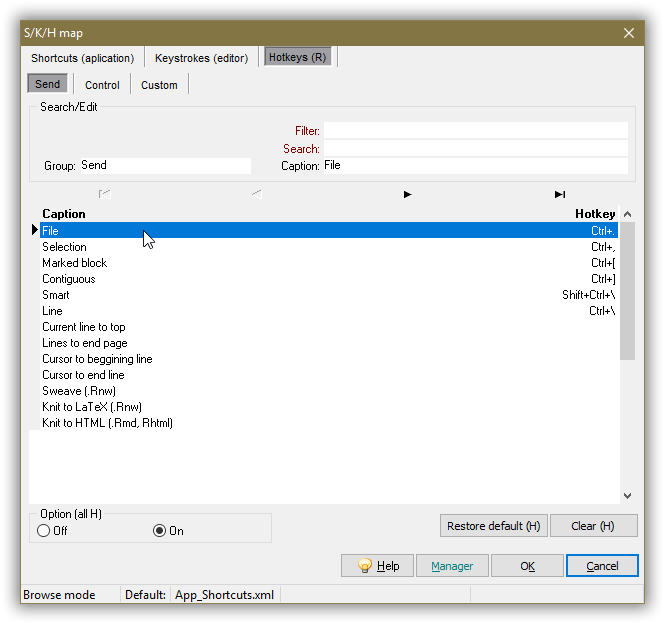
\includegraphics[scale=0.40]{./res/skh_map_rh_send_dlg.png}

Now, whenever you press \texttt{Ctrl + \textbackslash{}} the line you are on is sent to \RR{},
it is much faster than clicking with the mouse at the appropriate button and has the advantage
that you can send the line to \RR{} wherever is the focus of your present work in your computer.

You can also turn on and off the hotkeys by clicking the hotkeys on the status bar at the bottom of the Tinn-R screen.

Another important feature on the status bar is the \texttt{smNormal} (\texttt{s=selection, m=mode}) box.
This allows you to select a portion of a file.
Selecting it will change your options to \texttt{smLine} or \texttt{smColumn}.
The latter is helpful since it allows you to select columns within a file without having to carry the whole line with it.
Give it a try.

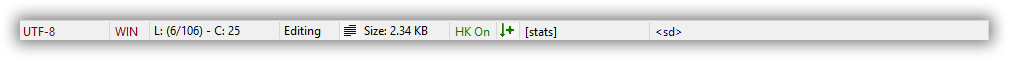
\includegraphics[scale=0.50]{./res/status_bar.png}

The first icons at the \RR{} task bar are related to different ways of sending instructions:
The whole file, selected parts, the clipboard content, block marked, contiguous lines, single line,
current line to bottom of page, parts of a line, Sweave and Knitr.
Those are helpful when you are dealing with long scripts,
and may very well enhance your programming efficiency.
Almost all of them have the option to send lines straight to \RR{} and with (echo=TRUE) option.


\includegraphics[scale=0.50]{./res/secrets_rtoolbar.png}
